%!TEX program = xelatex
\documentclass[table, aspectratio=169]{beamer}

\usetheme{Template}

\title{Search for New Heavy Gauge Bosons with ATLAS}
%\subtitle{Using all 2016 DS1 data from the 10/06 GRL}
\author{\underline{Ellis Kay}}
\institute{HEP Christmas Meeting 18/12/17}

\addtobeamertemplate{title page}{}{\color{TemplateGrey} \vspace{220pt}\begin{center}Supervisors: Uta Klein \& Carl Gwilliam\end{center}}

\date{ellis.kay@cern.ch}

\setcounter{showSlideNumbers}{1}

\begin{document}
	\setcounter{showProgressBar}{0}
	\setcounter{showSlideNumbers}{0}

	\frame{\titlepage}
	

	\setcounter{framenumber}{0}
	\setcounter{showProgressBar}{1}
	\setcounter{showSlideNumbers}{1}
	
	
	
	%%%%%%%%%%%%%%%%%%%%%%%%%%%%%%%%%%%%%%%%%%%%
	%%%%%%%%%%%%%%%%%  SLIDES  %%%%%%%%%%%%%%%%%
	%%%%%%%%%%%%%%%%%%%%%%%%%%%%%%%%%%%%%%%%%%%%
	
	\begin{frame}
	\frametitle{Motivation: W' Search}
	%\vspace{30pt}
		
	\cleft{.65}
	\vspace{10pt}
	\li{\wprime s are new heavy charged gauge bosons arising from extensions of electroweak symmetry.	}

	%\vspace{5pt}
	\li{Predicted in a wealth of BSM theories:}
		\lii{Little Higgs {\scriptsize \color{ATLASBlue} (hierarchy problem)}}
		\lii{Left-Right Symmetric {\scriptsize \color{ATLASBlue} (GUT)}}
		\lii{331 Models {\scriptsize \color{ATLASBlue} (3 quark families)}}
		\lii{Heavy Vector Triplet Models {\scriptsize \color{ATLASBlue} (many decay channels to combine)}}		
		
	
	\cright{.35}
	\vspace{30pt}
		\includegraphics[width=.95\linewidth]{plots/FEYNMAN/FeynmanWprime.png}

	\cend
	\vspace{5pt}	
	\li{We consider spin-1 s-channel \wprime resonances in the context of the Sequential Standard Model (SSM).}
		\lii{Same couplings to fermions as the SM W, TeV scale mass.}
		\lii{Neglect interference with SM W.}
		\lii{Very general benchmark model, others may be studied.}
	
	\li{I work on the electron channel.}
	
\end{frame}		
	
	
	
	
	
	
	
	

	
	

	
	

		
		
	
	\begin{frame}
	\frametitle{Analysis Strategy}

	\vspace{10pt}
	
	\li{Identify events with one high-\pt\, {\color{ATLASBlue}lepton} and large {\color{red}\met}.}
	
	\li{Search for deviations from SM in $\mt = \sqrt{2 {\color{ATLASBlue}\pt} {\color{red}\met} \big( 1 - \cos{\color{purple}\phi_{\ell\nu}} \big) }$.}
	
	\li{The dominant background is Charged Current Drell-Yan (CCDY) W $\rightarrow e\nu$.}
	
	\li{Final results from my 2015+2016 data analysis:}
	
	\vspace{-5pt}
	\begin{center}
		\includegraphics[width=\linewidth]{plots/KinematicsWithBGLabelled.png}

	\vspace{-10pt}
	
		{\scriptsize{{\color{green}Green bands }= systematics, shading = statistics}}
	
	\end{center}
	
	
 	\vspace{-20pt}


	
\end{frame}

		\begin{frame}
		\frametitle{Focus: Theoretical Modelling}
		\vspace{12pt}
		\li{Lack of knowledge of the parton structure of the proton is the dominant source of uncertainty in the \wprime\, \& \zprime\, searches.}
		
		\li{Mass dependent corrections are applied to Monte Carlo in order to correct to current theory knowledge.}
		
		\cleft{.5}
			\li{Shift signal \& dominant background to best theory.}
			\lii{Signal: 	QCD {\scriptsize(NNLO)}.}
			\lii{CCDY BG : QCD {\scriptsize(NNLO)} \& EW {\scriptsize(NLO)}.}
			
			\li{Apply theoretical uncertainties for background predictions:}
			\lii{PDF \& $\alpha_{S}$ uncertainty for nominal PDF.}
			\lii{PDF choice uncertainty.}
		
		\vspace{-10pt}
		\begin{center}
		
		{\scriptsize{We calculate these uncertainties for the DY process and distribute them in widely used ATLAS tools.}}			\end{center}
		
		\cright{.5}
			\centering
			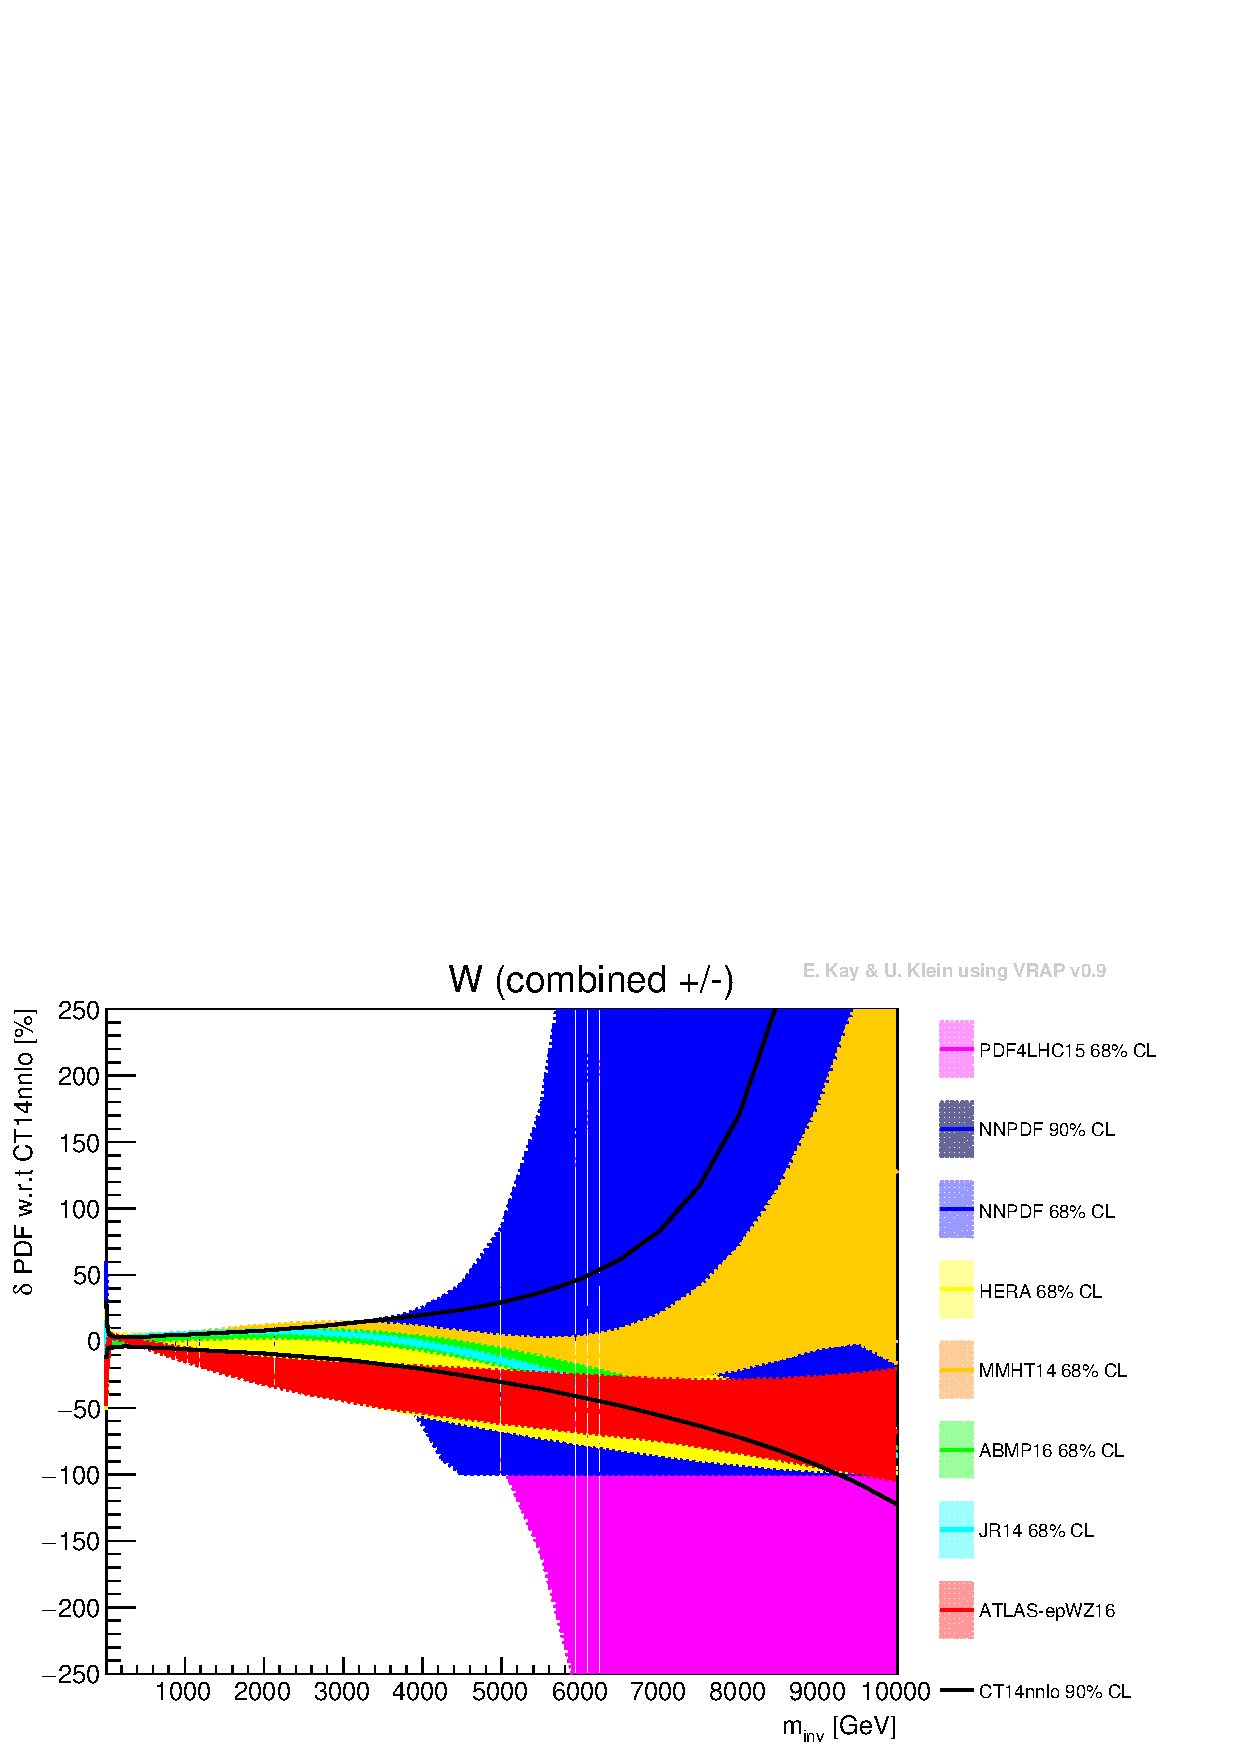
\includegraphics[height=\linewidth,angle=270]{plots/SUMMARY_ALLNEW/Wcomb.pdf}

		\cend
		
	
\end{frame}	
	
	\begin{frame}
	\frametitle{Published Results}
	\vspace{15pt}
	\li{Both \href{https://arxiv.org/abs/1707.02424}{{\color{ATLASBlue}\underline{\zprime}}} (JHEP) and \href{https://arxiv.org/abs/1706.04786}{{\color{ATLASBlue}\underline{\wprime}}}\, 2015+2016 (36.1 fb\textsuperscript{-1}) analyses are now published on arXiv!}
	\cleft{.5}
	
	\includegraphics[width=\linewidth]{plots/WprimeLimit_arXiv.png}
	\cright{.5}
	\includegraphics[width=\linewidth]{plots/DileptonLimit_arXiv.png}
	\cend

\vspace{-10pt}
	\li{Both set limits using the Bayesian Analysis Toolkit (BAT).}
	\li{Exclude $W'_{SSM} <$ 5.1 TeV, $Z'_{\chi} (E_{6}) <$ 4.1 TeV!}
\end{frame}
	
	\begin{frame}
	\frametitle{NEW: Heavy Vector Triplet Model}
	
	\cleft{.5}
	\vspace{10pt}
	\li{In general effective theories with an extended gauge sector, new particles can arise in multiplets of Lorentz and gauge quantum numbers.}
	\lii{Where each multiplet has a well defined phenomenology.}
	\li{We consider a \href{https://arxiv.org/abs/1402.4431}{{\color{ATLASBlue}\underline{Heavy Vector Triplet}}} $\mathcal{W}$.}
	\lii{Predicts two charged \wprime s and an uncharged \zprime.}
	\lii{Three couplings: to leptons $g_{l}$, quarks $g_{q}$ and Higgs $g_{H}$ (also denoted $g_{\phi}$).}
	\lii{Many available decay channels to combine.}
	
	\li{Limits are set in a coupling plane.}

	\cright{.5}
	\begin{center}
	\includegraphics[width=\linewidth]{plots/HVTSummary.png}\\
	\scriptsize{  \href{https://arxiv.org/abs/1211.2229}{{\color{ATLASBlue}\underline{Manuel P\'erez-Victoria}}} }
	
	\end{center}
	\cend
	
	
\end{frame}
	
	\begin{frame}
		\frametitle{Combining W' \& Z'}
		\vspace{20pt}
%		\li{Both \href{https://arxiv.org/abs/1707.02424}{{\color{ATLASBlue}\underline{\zprime}}} (JHEP) and \href{https://arxiv.org/abs/1706.04786}{{\color{ATLASBlue}\underline{\wprime}}}\, 2015+2016 (36.1 fb\textsuperscript{-1}) analyses are now published on arXiv!}
		
		\li{There is an \href{https://svnweb.cern.ch/cern/wsvn/atlasphys-exo/Physics/Exotic/LPX/ZpWpComb/Run2_2016/Notes/SupportNote/trunk/wpzpCombinationSupportNote2016.pdf}{{\color{ATLASBlue}\underline{ongoing effort}}}	to combine our W' and Z' results.}	
		
		\li{Results will also be combined with decays to dibosons (VV/VH).}
		\lii{Using this Heavy Vector Triplet model.}
		
	
		

		\begin{center}
		
		\includegraphics[width=.9\linewidth]{plots/CombinedLimitsLabelled.png}


		\vspace{-10pt}
		Plots from W. Fisher (\href{https://cds.cern.ch/record/2273871}{{\color{ATLASBlue}\underline{diboson resonance search}}})
	\end{center}
	%\cend
	
	
		%\vspace{-20pt}
		
	\end{frame}
	
	\begin{frame}
	\frametitle{Statistical Tools}
	\vspace{10pt}
	
	\li{Original $\ell\ell$ and $\ell\nu$ analyses used the Bayesian Analysis Toolkit for statistical analysis.}
	
	\li{Diboson analyses set Frequentist limits $\rightarrow$ \wprime\, \& \zprime must be moved to compatible tools.}
	
	\li{Now using two adapted ATLAS frameworks to calculate limits with both asymptotic calculations \& pseudo-experiments (PEs).}
	\lii{PEs appear more stable for these high mass searches where statistics are low.}
	\lii{Computationally expensive but performed quickly thanks to heavy parallelisation.}
	
	\li{I have been responsible for writing the statistical analysis code, performing detailed validation checks and providing results for the ATLAS note.}
	
	\li{There is generally a good agreement between Bayesian \& Frequentist frameworks.}
	\lii{Some differences for lowest mass points $\lesssim$ 600-800 GeV caused by different treatment of MC statistical error.}
		
	\li{Group is satisfied that our tools are validated, we are ready to process W' \& Z' channels in the context of HVT.}
	
	
	
\end{frame}


\begin{frame}
	\frametitle{Statistical Tools: Validation}
	\cleft{.35}
	\begin{center}
	\includegraphics[width=\linewidth]{plots/Zll_SystsNew10000PE_2017-11-03/Zll_SystsNew10000PE_2017-11-03_Zll_Systs_ObsRatioBAT_Toys.eps}
\\	\includegraphics[width=\linewidth]{plots/Zll_SystsNew10000PE_2017-11-03/Zll_SystsNew10000PE_2017-11-03_Zll_Systs_ExpRatioBAT_Toys.eps}
	\end{center}
	\cright{.35}	
	\begin{center}
	\includegraphics[width=\linewidth]{plots/Wlnu_SystsNew10000PE_2017-11-07/Wlnu_SystsNew10000PE_2017-11-07_Wlnu_Systs_ObsRatioBAT_Toys.eps}
\\	\includegraphics[width=\linewidth]{plots/Wlnu_SystsNew10000PE_2017-11-07/Wlnu_SystsNew10000PE_2017-11-07_Wlnu_Systs_ExpRatioBAT_Toys.eps}
	\end{center}
		
	\cright{.3}
	\vspace{30pt}
	\li{Blue dashed line: \\ Bayesian}
	\li{Black line: \\ Frequentist (PEs)}
	
	\vspace{20pt}
	
	\li{Top row = \\ observed limits}
	\li{Bottom row = \\ expected limits}
	
	\cend
	
\end{frame}
	
	\begin{frame}
	\frametitle{First HVT Limits}
	\vspace{15pt}
	\cleft{.5}
		\includegraphics[width=\linewidth]{plots/VprimeHVT_g0_Zt05_Wt08_WZlvll_Wlnu_Zll_Systs.eps}
	\vspace{-20pt}
	{\scriptsize{
	\cleft{.2}
	\cright{.4}
	{\color{blue} Z':\\ Observed = 4.45 TeV\\Expected = 4.39 TeV\\}
	
	{\color{red} W':\\Observed = 4.49 TeV\\Expected = 4.63 TeV\\ }
	\cright{.4}
	\vspace{15pt}
	{\color{magenta} W'/Z':\\Observed = 4.83 TeV\\Expected = 4.93 TeV\\ }	
	\cend
	}}
	
	\cright{.5}
	\vspace{20pt}
	\li{First real combination of W' \& Z' results.}
	\lii{Using asymptotic calculations.}
	\lii{With systematics, including correlations \& decorrelations.}
	
	\li{We present these limits as $\frac{\sigma}{\sigma_{HVT}}$ to remove model dependence for diboson limits.}
	
	\li{Overlay individual channels to show improvement provided by combination.}	
	
	\li{Still working to fully understand these.}
	\lii{Will check diagnostic plots, possibly compare to PEs.}

		
	\cend
	
\end{frame}
	
	\begin{frame}
	\frametitle{Conclusion \& Outlook}
	\vspace{10pt}
		
	\li{Both \wprime\, \& \zprime\, 2015+2016 (36.1 fb\textsuperscript{-1}) analyses are complete.}
		\lii{With CONF notes at summer conferences and published papers on arXiv.}
	\li{Upper and lower uncertainties in cross sections for all modern NNLO PDF sets have been calculated, following various prescriptions.}
		\lii{Results are used in official ATLAS tools.}

	\li{Frequentist limit setting code for W' \& Z' (SSM + HVT) has been set up (asymptotic \& PEs)}.


	\li{Contributing studies to novel \wprime / \zprime / diboson combination effort (following discussions which took place during Exotics/SUSY workshop, Bucharest). }
	
	\li{Now working on exclusion limits in a 2D coupling plane for \wprime/\zprime.}
	
	
	\vspace{10pt}
	\textbf{Ongoing / TO DO:}
	\li{Continue making contributions to the combination effort, aiming towards an ATLAS paper.}
	\li{Continue writing thesis.}	
	
\end{frame}
	
	%%%%%%%%%%%%%%%%%%%%%%%%%%%%%%%%%%%%%%%%%%%%
	%%%%%%%%%%%%%%%%%  BACKUP  %%%%%%%%%%%%%%%%%
	%%%%%%%%%%%%%%%%%%%%%%%%%%%%%%%%%%%%%%%%%%%%
	\beginbackup
	\setcounter{showSlideTotal}{0}
	\section{Backup}
	\begin{frame}
	\frametitle{Selections}
		\scriptsize{
			\include{plots/selections_elec_muon}
		} % end tiny font
		
\end{frame}
	\begin{frame}
	\frametitle{Signal \& Background Modelling}
	\vspace{15pt}
	\cleft{.4}
	%\vspace{10pt}
	
     Signal:
	\li{``Flat'' W' signal samples are reweighted to a desired \wprime pole mass. }
	\vspace{8pt}
	\hspace{10pt}\includegraphics[width=.9\linewidth]{plots/FEYNMAN/ExamplesUnboxed.png}
	\cright{.3}
	\vspace{10pt}
	 \includegraphics[width=\linewidth]{plots/SignalTemplates_truth.eps}
	\cright{.3}
	\vspace{10pt}
	 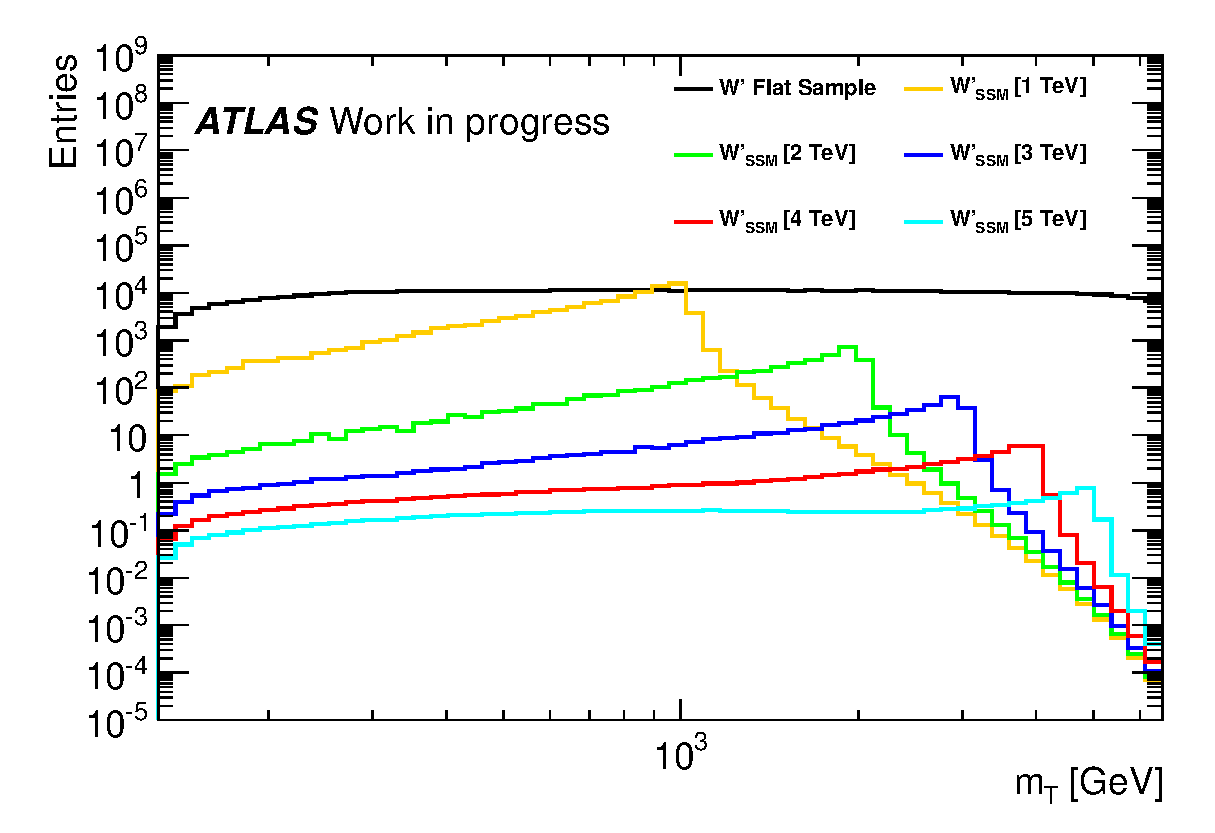
\includegraphics[width=\linewidth]{plots/SignalTemplates.eps}			
	\cend
	\vspace{5pt}
	\cleft{.6}
	Backgrounds:
	\li{Charged Current Drell-Yan $W \rightarrow e \nu$\ {\color{ATLASBlue}(mass-binned)}. \\{\footnotesize This is the \underline{dominant} background}}
	\li{Neutral Current Drell-Yan $Z \rightarrow \ell \ell$ {\color{ATLASBlue}(mass-binned)}. }
	\li{Top ($t\bar{t}$ \& single top) {\color{ATLASBlue}(inclusive + fit)}.}
	\li{Diboson {\color{ATLASBlue}(inclusive + fit)}.}
	
	\li{Multijet background {\color{ATLASBlue}(data-driven 	method + fit)}.}
	\cright{.4}
	
     
   	\includegraphics[width=.9\linewidth]{plots/h_signal_electron_mt_CCDYplus.eps}
   
     
    
   \cend

\end{frame}		
	\begin{frame}
	
		\frametitle{Signal Sample Reweighting}
		\vspace{30pt}
		
		\begin{itemize}
		
		\item A `flat' signal sample is produced by removing the Breit-Wigner term from the cross section calculation in Pythia and fitting the resulting mass spectrum to smooth out bumps. 
		\item These terms must be replaced using the desired pole mass in order to obtain signal peaks.
		\end{itemize}
		
\begin{equation*}
	\Gamma = \frac{1}{\sin^{2}\Theta_{W} \times ( \alpha_{EM}(m_{Z})^{-1} + 1.45 log( \frac{m_{Z}}{M}) )} \times \frac{3 + ( 1 + \frac{rtW}{2}) \times ( 1 - rtW )^{2} }{4}
\end{equation*}



\begin{equation*}
	W_{BW} = \frac{1}{(m_{\ell\nu}^{2} - M^{2})^{2} + (m_{\ell\nu}^{2} \times \Gamma)^{2}}
\end{equation*}

Where M = desired polemass, $m_{\ell\nu}$ = invariant mass and $rtW = \Big(\frac{m_{t}}{M}\Big)^{2}$
		
		
%	\begin{itemize}
%		\item 
%		
%	
%\end{itemize}			
		
		
	
	\end{frame}
	
	
		\begin{frame}
	
		\frametitle{Signal Sample Reweighting}
		
		
	
		
		\li{$m_{\ell\nu}$-dependent weights are calculated and applied to the signal sample. }
		
		\begin{equation*}
  w = 
  \begin{cases}
    10^{12} \times 102.77 \exp\Big( -11.5 \frac{m_{\ell\nu}}{\sqrt{s}}\Big) \times W_{BW} & \text{if}\,\, m_{\ell\nu} < 299\, \text{GeV},\\
    10^{12} \times \exp\Big( -16.1 \frac{m_{\ell\nu}}{\sqrt{s}}\Big) \times \Big(\frac{m_{\ell\nu}}{\sqrt{s}}\Big)^{1.2} \times W_{BW} & \text{if}\,\, m_{\ell\nu} \geqslant 299\, \text{GeV}, m_{\ell\nu} < 3003\, \text{GeV},\\
    10^{12} \times 1.8675 \exp\Big( -31.7 \frac{m_{\ell\nu}}{\sqrt{s}}\Big) \times \Big(\frac{m_{\ell\nu}}{\sqrt{s}}\Big)^{4.6} \times W_{BW} & \text{if}\,\, m_{\ell\nu} \geqslant 3003\, \text{GeV}.
  \end{cases}
\end{equation*}

		
	
	\end{frame}
	\begin{frame}
	\frametitle{``Fake'' Lepton Background}
	
	\vspace{15pt}
	\li{QCD jet production ($\rightarrow$ ``fake'' leptons) ill described by MC $\rightarrow$ use the Matrix Method.}
		\lii{Exploits the different
probabilities for ``real'' and ``fake'' leptons to
pass from ``loose'' to ``tight'' cuts}
		\lii{Using {\color{orange}measurable} quantities to calculate {\color{purple}truth} quantities}
			
		\vspace{-5pt}
		%\begin{center}\makebox[.7\textwidth][c]{%
		\begin{minipage}{.5\linewidth}
			\begin{equation*}
			\psBox{orange!30}{
  		  		\begin{pmatrix} 
				N_{T} \\
				N_{L} 
				\end{pmatrix}
				}=
				\begin{pmatrix}
				\epsilon_{R} & \epsilon_{F} \\
				1 - \epsilon_{R} & 1 - \epsilon_{F}
				\end{pmatrix}
				\psBox{purple!30}{
				\begin{pmatrix}
				N_{R} \\
				N_{F}
				\end{pmatrix}
				}
 		 	\end{equation*} 
		\end{minipage}\hfill
		\begin{minipage}{.4\linewidth}
			\begin{equation*}
			\boxed{
 				\epsilon_{F} = \frac{N^{fake}_{tight}}{N^{fake}_{loose}}, \, \,  
 				\epsilon_{R} = \frac{N^{real}_{tight}}{N^{real}_{loose}}
 				}
  			\end{equation*}
		\end{minipage}
		\vspace{10pt}
		\cleft{.25}
		\vspace{10pt}
		\li{From the first line:}
		\cright{.75}
		\begin{equation*}
  	\begingroup
  		\color{ATLASBlue_lighter}\overbrace{\color{black}				\highlight[ATLASBlue_lighter]{N_{T}}}^{\mathclap{\text{\color{ATLASBlue}signal selection}}}
  %\highlight[ATLASBlue_lighter]{N_{T}} 
  \endgroup
  \,\,= \,\,
  \begingroup
  \color{highgreen}\underbrace{\color{black}\highlight[highgreen]{\epsilon_{R}N_{R}}}_{\mathclap{\text{\color{green}contribution from real electrons}}}
  %\highlight[highgreen]{\epsilon_{R}N_{R}} 
  \endgroup
  \,\,+ \,\,
  \begingroup
  \color{highred}\overbrace{\color{black}\highlight[highred]{\epsilon_{F}N_{F}}}^{\mathclap{\text{\color{red}contribution from fake electrons}}}
  %\highlight[highred]{\epsilon_{F}N_{F}}
  \endgroup \,\,\, \, ,
\end{equation*}
\cend

\li{Inverting matrix yields ``fake'' component in data (tight selection):}
\vspace{10pt}
		\begin{equation*}
			\epsilon_{F}N_{F} = \frac{\epsilon_{F}}{\epsilon_{R} - \epsilon_{F}} \big[ \epsilon_{R}(N_{L} + N_{T}) - N_{T} \big]	
		\end{equation*}
		
		\vspace{-10pt}
\end{frame}
	

\begin{frame}
	\frametitle{``Fake'' Lepton Background}
	\vspace{10pt}
	\li{Loose Selection:}
		\lii{{\bfseries $e$:} signal selection except LHTight ID \& isolation $\rightarrow$ only LHMedium / LHLoose. }
		\lii{{\bfseries $\mu$:} signal selection except isolation}			
	\li{Tight Selection: same as signal selection.}

	\vspace{20pt}
		\begin{minipage}{0.44\textwidth}
			\begin{center}
				{\bfseries REAL}
			\end{center}
		\end{minipage}
		\begin{minipage}{0.52\textwidth}
			\begin{center}
				{\bfseries FAKE}
			\end{center}
		\end{minipage}\par\medskip
		\begin{minipage}{0.44\textwidth}
			\begin{itemize}
				\item Count real $\ell$ candidates passing selections.
				\item Estimate $\epsilon_{R}$ with W MC and truth matching ($\Delta$R < 0.2).
				\item \pt\, and $\eta$ dependency $\rightarrow$ 2D binning.
			\end{itemize}
		\end{minipage}
		\begin{minipage}{0.52\textwidth}
			\begin{itemize}
				\item Calculate using data.
				\item Cut to suppress genuine $\ell$\, from W \& Z.
				\item Account for contamination with real $\ell$\, with MC {\footnotesize (subtract real-electron dilution from fake rate)}.
				\item Binned in \pt\, and $\abs{\Delta\phi_{e,\met} }$.
			\end{itemize}
		\end{minipage}
	
\end{frame}		


\begin{frame}
	\frametitle{Fake Rates}
	
	\cleft{.5}
	\begin{center}
		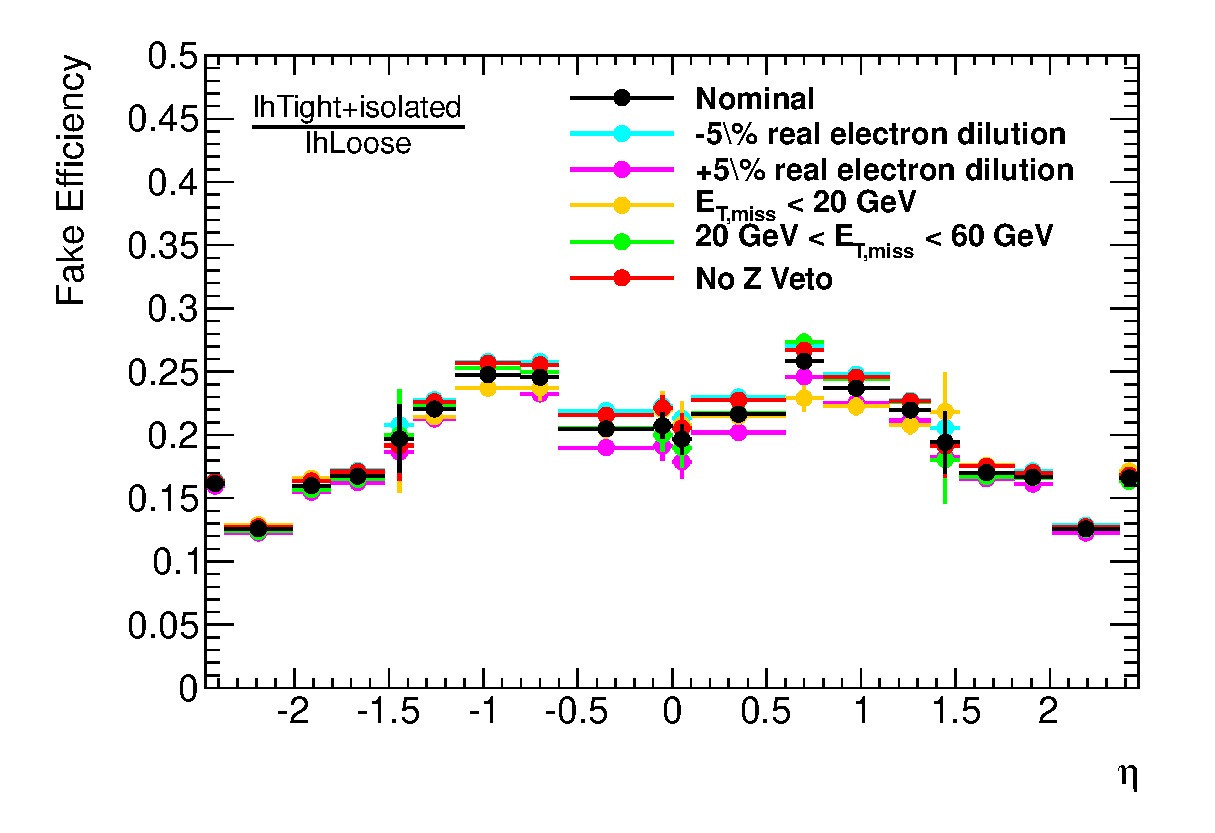
\includegraphics[width=.7\linewidth]{plots/RealsFakesMine/TL_FakeRate_eta_F.eps}\\
		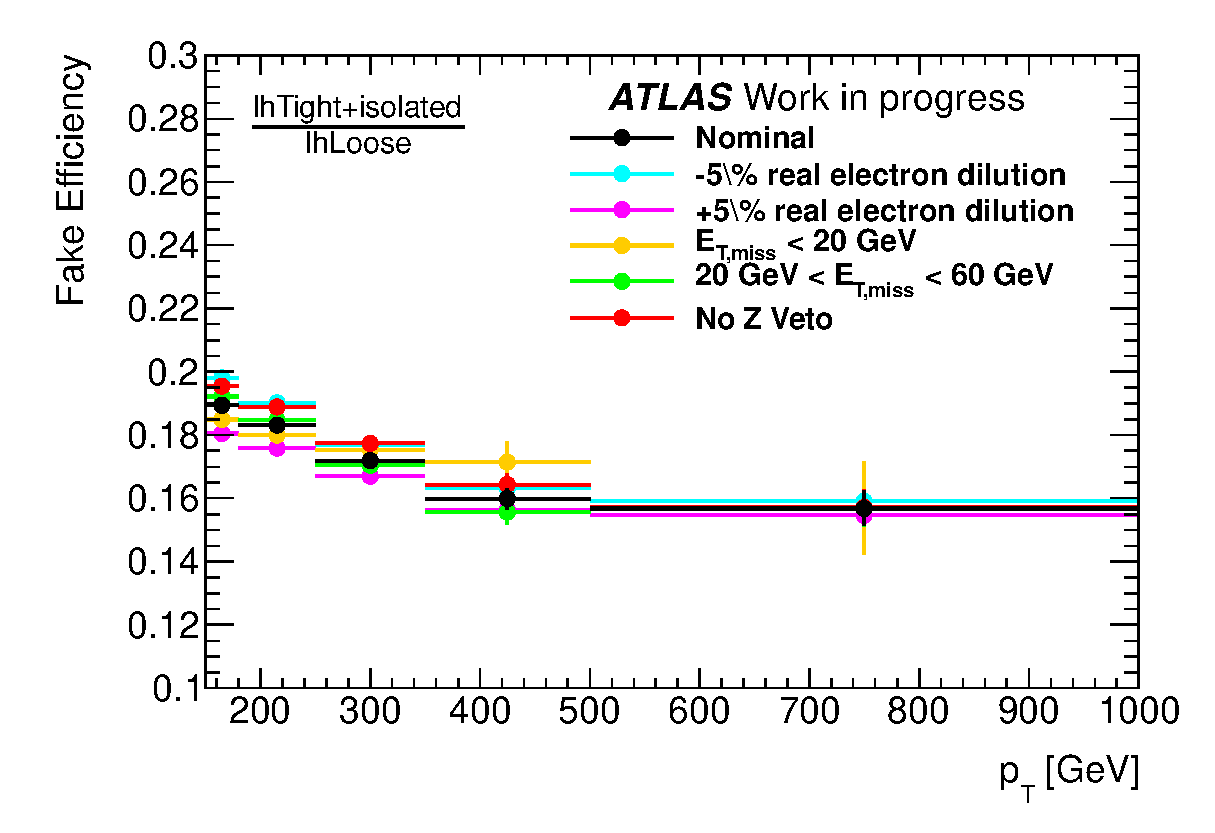
\includegraphics[width=.7\linewidth]{plots/RealsFakesMine/TL_FakeRate_pt_F.eps}
	\end{center}
	\cright{.5}
	\begin{center}
		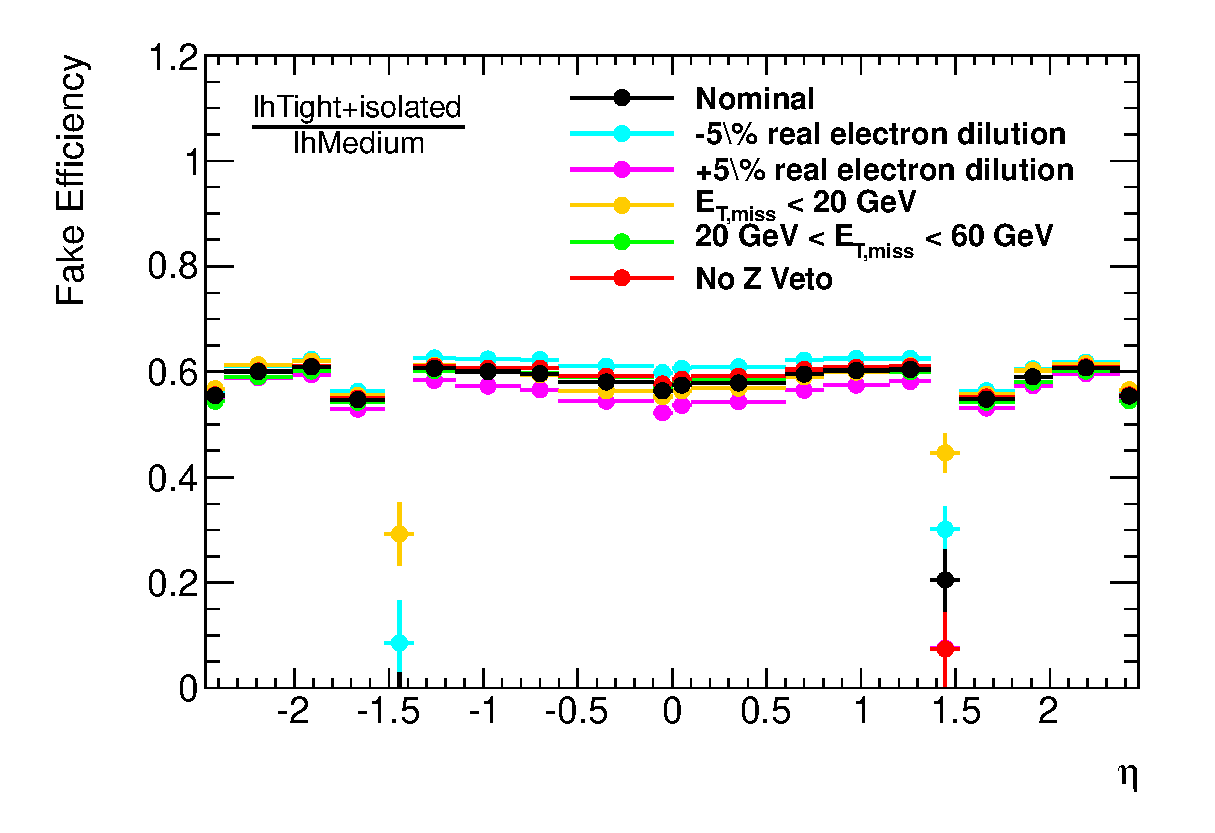
\includegraphics[width=.7\linewidth]{plots/RealsFakesMine/TM_FakeRate_eta_F.eps}\\
		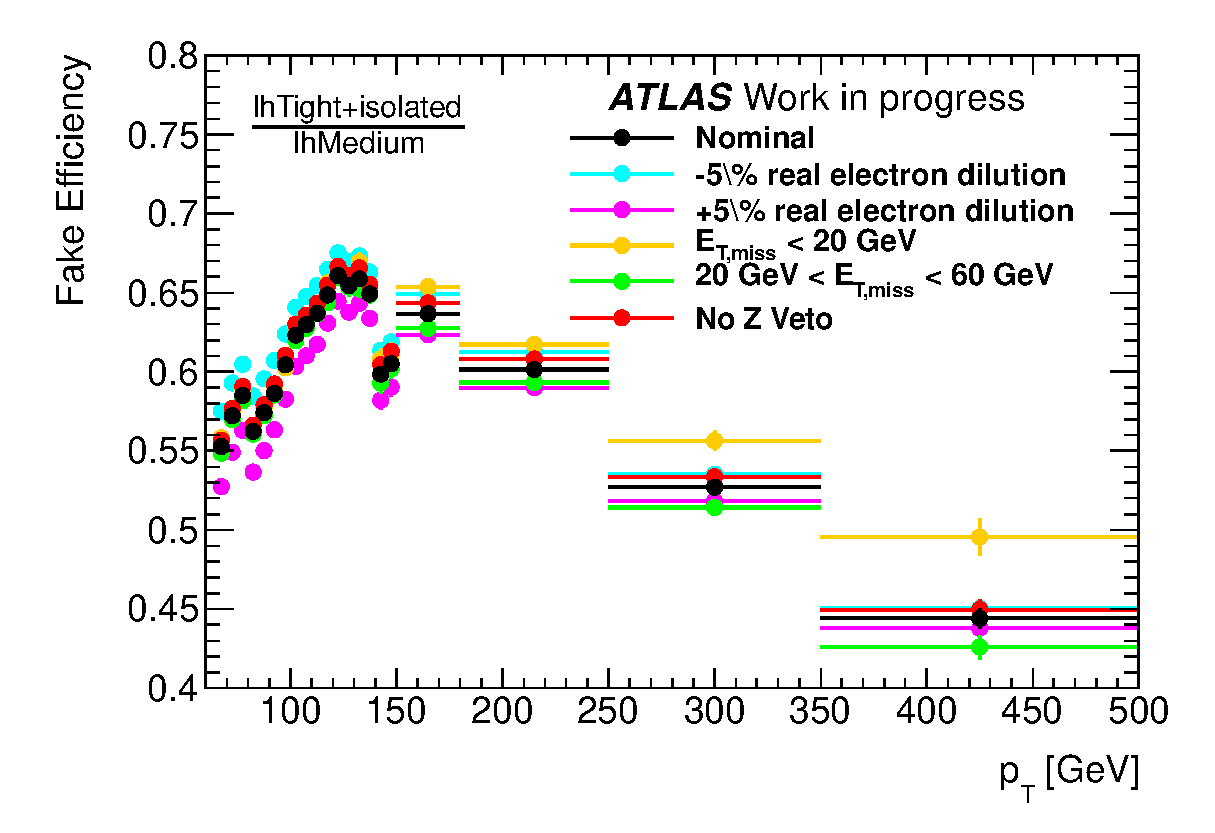
\includegraphics[width=.7\linewidth]{plots/RealsFakesMine/TM_FakeRate_pt_F.eps}
	\end{center}
	\cend
\end{frame}

\begin{frame}
	\frametitle{Real Rates}
	
	\cleft{.25}
	\cright{.5}
	\begin{center}
		\includegraphics[width=.7\linewidth]{plots/RealsFakesMine/ALL_RealRate_eta_F.eps}
	\end{center}
	\cright{.25}
	\cend
	\vspace{-10pt}
	\cleft{.5}
	\begin{center}
		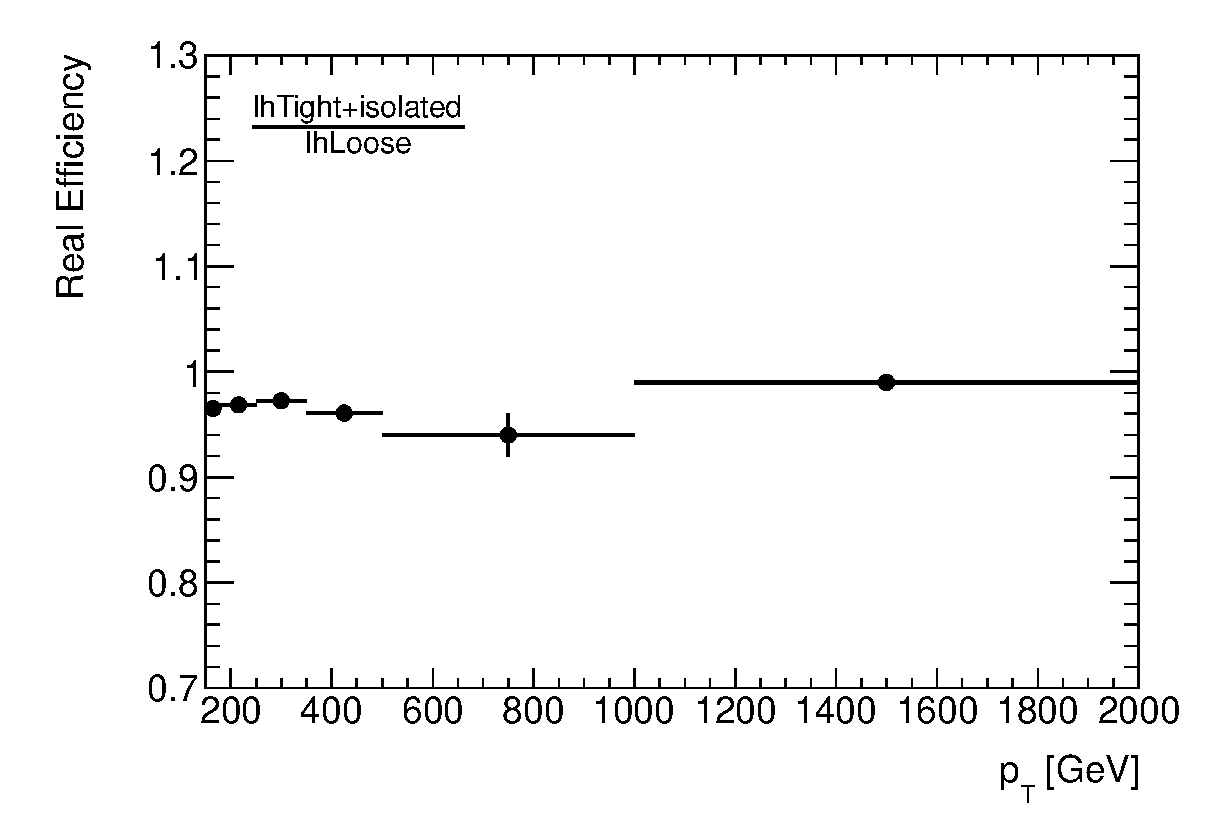
\includegraphics[width=.7\linewidth]{plots/RealsFakesMine/TL_RealRate_pt_F.eps}
	\end{center}
	\cright{.5}
	\begin{center}
		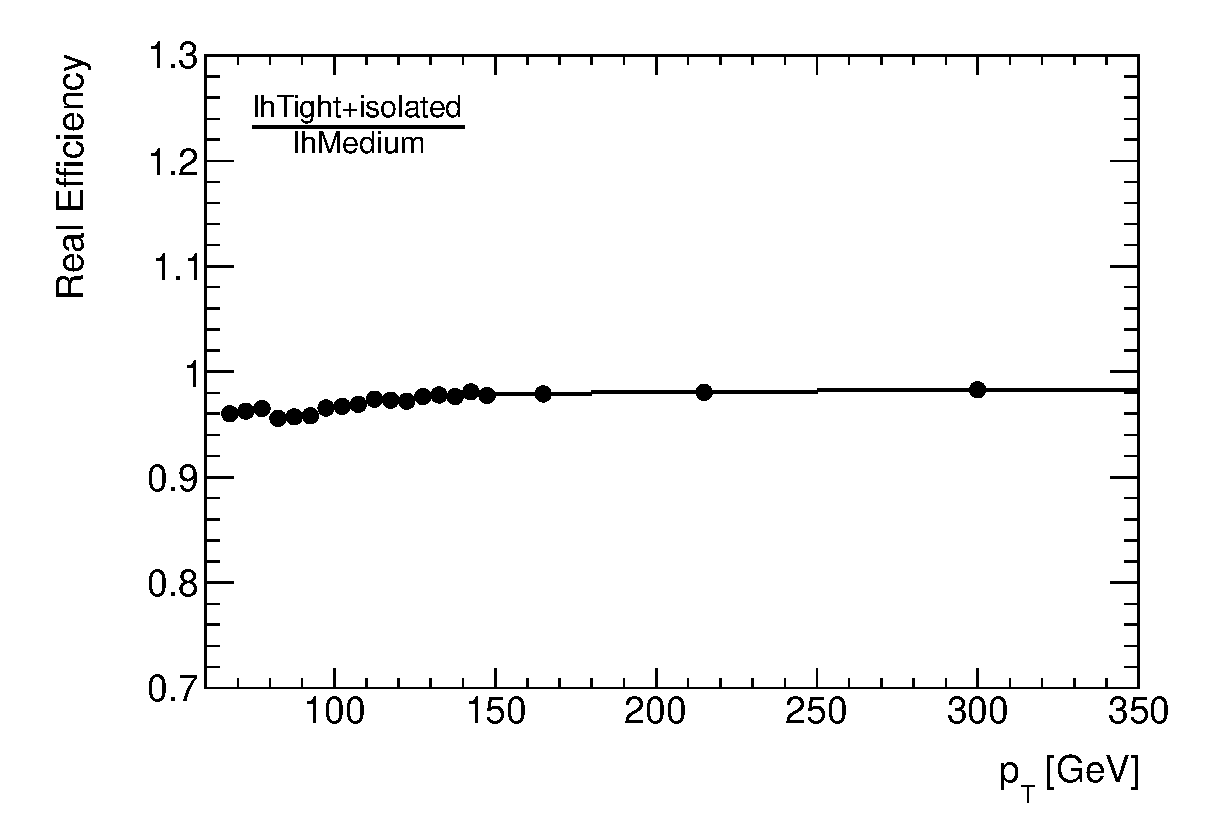
\includegraphics[width=.7\linewidth]{plots/RealsFakesMine/TM_RealRate_pt_F.eps}
	\end{center}
	\cend
\end{frame}
	\begin{frame}
	\frametitle{Background Extrapolation}
	
	\li{Insufficient statistics at high $m_{T}$ for \underline{inclusive} top ($t\bar{t} $ \& single top) and diboson samples.}
	\li{Extrapolate fits using two functions:}	
	\begin{center}\makebox[.7\textwidth][c]{%
	\begin{minipage}{.2\textwidth}
		\begin{equation*}
  		  \frac{dN}{dm_{T}} = am_{T}^{b + c log(m_{T})}
 		 \end{equation*}
	\end{minipage}\hfill
	\begin{minipage}{.2\textwidth}
		\begin{equation*}
 			\frac{dN}{dm_{T}} = \frac{a}{ \big(m_{T} + b\big)^{c}}
  		\end{equation*}
	\end{minipage}
	} \end{center}


\li{Systematics variations: vary start and end point for range of both fit functions.}
\lii{Central value: best $\frac{\chi^{2}}{N_{d.o.f}}$.}
\lii{Uncertainty: Envelope of all fits.}
\lii{Replace MC results with fits above chosen stitching point.}

\end{frame}


\begin{frame}
	\frametitle{Background Extrapolation}
	
	\cleft{.5}
	\vspace{20pt}
	\li{For QCD - select fits which satisfy:}
	
	\begin{equation*}
		\frac{1}{N_{bins}}\sum_{b>b_{s}}^{N_{b}^{MM} \neq 0} \frac{\big( N_{b}^{MM} - N_{b}^{fit} \big)^{2}}{\sigma_{b}^{2}} < 1.5
	\end{equation*}
	\li{Central value: fit with minimal value.}
	
	\cright{.5}
	\begin{center}
	
	\begin{tikzpicture}
            	\node[anchor=south west,inner sep=0] (image) at (0,0) {\includegraphics[width=.65\linewidth]{plots/FittedBG/FitSummaryExtrapolation_h_QCD_electron_mt_elec_QCD.eps} };
            	
            	\begin{scope}[x={(image.south east)},y={(image.north west)}]
            	
            	\node at (.78,.84) [preaction={fill, ATLASBlue}, font={\tiny\bfseries}, text=white] {QCD};
            	
        		\end{scope}
    \end{tikzpicture}	
		
	\end{center}
	\cend
	\vspace{-10pt}
	\cleft{.5}
	
	\begin{center}
	
	\begin{tikzpicture}
            	\node[anchor=south west,inner sep=0] (image) at (0,0) {\includegraphics[width=.65\linewidth]{plots/FittedBG/FitSummaryExtrapolation_h_signal_electron_mt_elec_DB.eps} };
            	
            	\begin{scope}[x={(image.south east)},y={(image.north west)}]
            	
            	\node at (.78,.84) [preaction={fill, ATLASBlue}, font={\tiny\bfseries}, text=white] {Diboson};
            	
        		\end{scope}
    \end{tikzpicture}	
		
	\end{center}
	
	\cright{.5}
	
	\begin{center}
	
	\begin{tikzpicture}
            	\node[anchor=south west,inner sep=0] (image) at (0,0) {\includegraphics[width=.65\linewidth]{plots/FittedBG/FitSummaryExtrapolation_h_signal_electron_mt_elec_TTST.eps} };
            	
            	\begin{scope}[x={(image.south east)},y={(image.north west)}]
            	
            	\node at (.78,.84) [preaction={fill, ATLASBlue}, font={\tiny\bfseries}, text=white] {Top};
            	
        		\end{scope}
    \end{tikzpicture}	
		
	\end{center}
	
	\cend
\end{frame}
	\begin{frame}
	\frametitle{Event Yields}
	
	\vspace{20pt}
	\li{Yields are monitored to check for strange behaviour in new runs (with possible high \mt\, candidates!).}
	\li{Non-linear behaviour appears to be attributed to pileup ($<\mu>$).}
	%\item Average pile-up per run is plotted - explains 2016 non-linear behaviour.

\cleft{.7}
	
		\includegraphics[width=\linewidth]{plots/yield_std_DATA16.eps}
		\vspace{2pt}
		\includegraphics[width=\linewidth]{plots/periods_avgmu_DATA16.eps}


\cright{.3}
	\includegraphics[width=\linewidth]{plots/mu_vs_yield_DATA15.eps}
		\vspace{2pt}
		\includegraphics[width=\linewidth]{plots/mu_vs_yield_DATA16.eps}
\cend

\end{frame}	
	\begin{frame}
	\frametitle{W' Systematics}
	%\vspace{10pt}
	\cleft{.5}
		\begin{center}
		\includegraphics[width=.7\linewidth]{plots/sysplots/exptest_electron_mt.eps}\\
		\includegraphics[width=.7\linewidth]{plots/sysplots/theotest_electron_mt.eps}	
		\end{center}
	\cright{.5}
		\begin{center}
		\includegraphics[width=.7\linewidth]{plots/sysplots/qcdtest_electron_mt.eps}\\
		\includegraphics[width=.7\linewidth]{plots/sysplots/extraptest_electron_mt.eps}	
		\end{center}
	\cend
\end{frame}
	\begin{frame}
		\frametitle{Results}
		\cleft{.5}
		\includegraphics[width=\linewidth]{plots/Wenu_EllisSyts100000PE_2017-12-06_Wenu_spline.eps}
		
		\cright{.5}
		\vspace{20pt}
		\li{Limits set using 100,000 pseudo-experiments.}
		\vspace{20pt}
		\input{plots/LIMITS_Wenu_EllisSyts100000PE_2017-12-06_Toys}
		\cend
	\end{frame}
	\begin{frame}
	\frametitle{MC PDFs}
	
	\li {Some PDF sets are produced using the Monte Carlo methodology, whereby a number of pseudodata replicas are generated around the nominal value. }
	\li {Central curves are constructed by taking a simple mean of all of these replicas for each mass point. }
	\li {Upper and lower uncertainties are calculated at 90\% CL and 68\% CL by excluding the appropriate number of highest and lowest replicas and then taking the maximum and minimum replica values for each mass bin. }
			
	\vspace{10pt}
	\li {NNPDF 3.0 and PDF4LHC15 both have MC PDF sets.}
	
\end{frame}





\begin{frame}
	\frametitle{MC PDFs (2)}
	
	\cleft{.48}
	\vspace{10pt}
	\li {In some cases, many replicas have negative cross sections, leading to a negative central value. }
	\lii {This is symptomatic of the absence of PDF data at high x where cross sections are driven to extremely low values.}
	\lii {Following the advice of NNPDF authors, negative replicas are set to zero.}
	\lii {For NNPDF a 100 replica set proved too small, with \textasciitilde 50\% of the replica values going negative.}
	\lii {A 1000 replica set is needed to provide at least \textasciitilde 500 positive replicas.}
	
	\cright{.52}
	\vspace{5pt}
	\begin{center}
	
	
	\includegraphics[height=\linewidth, angle=270]{plots/PDFs/NNPDF_Wcomb_allpos_posneg.pdf}
	{ \color{ATLASBlue} \scriptsize posneg = before setting negative replicas to zero.}\\
	{ \color{ATLASBlue}\scriptsize allpos = after setting negative replicas to zero.} \\
	{ \color{ATLASBlue}\scriptsize `median' = median value excluding zeros.}
	
	\end{center}
	\cend
	
\end{frame}
	\begin{frame}
	\frametitle{Hessian PDFs}
	
	\li {PDF sets with Hessian-type errors are provided as a set of orthogonal `eigenvectors' (EVs) which are formed by varying the central PDF values by their systematic uncertainties.}
	
	
	
	
	
	\vspace{5pt}
	\li {In the asymmetric case, EVs consist of pairs of values which form the up and down uncertainties: }
	\vspace{5pt}
	\cleft{.6}
	\begin{equation*} \label{eq:hessup}
\Delta\sigma^{+} = \sqrt{\sum_{i=1}^{N_{eig}}\bigg[ \text{max}\big(\sigma^{+}_{i} - \sigma_{0}, \sigma^{-}_{i} - \sigma_{0}, 0\big) \bigg]^{2} }
\end{equation*}

\begin{equation*} \label{eq:hessdown}
\Delta\sigma^{-} = \sqrt{\sum_{i=1}^{N_{eig}}\bigg[ \text{max}\big(\sigma_{0} - \sigma^{+}_{i}, \sigma_{0} - \sigma^{-}_{i}, 0\big) \bigg]^{2} }
\end{equation*}

	\cright{.4}
	\vspace{20pt}
	$N_{eig}$ - no. of PDF eigenvectors\\
	$\sigma_{0}$ - central value PDF\\
	$\sigma^{+}_{i}$ - higher value of the i\textsuperscript{th} PDF EV \\ 
	$\sigma^{-}_{i}$ - lower value of the i\textsuperscript{th} PDF EV	
	
	\cend
	
	
\end{frame}








\begin{frame}
	\frametitle{Hessian PDFs (2)}
	
	\li {For the symmetric case, variations are not paired. }
	\li {In this case, the symmetric error for each EV is simply the difference between the variation and the nominal value:}
	\vspace{5pt}
	
	\begin{equation*} \label{eq:hessavg_symm}
\Delta\sigma^{symm} = \sqrt{\sum_{i=1}^{N_{eig}}\big[ \sigma_{i} - \sigma_{0} \big]^{2} }
\end{equation*}

\li {Asymmetric sets studied here include: CT14, HERA 2.0, MMHT2014, ATLASep-WZ16.}
\li {Symmetric sets studied here include: CT14\_EWbun (our reduced set), ABM (12 \& 16), PDF4LHC15, JR14.}

\vspace{10pt}
\li {Overall error curves are constructed by summing all of the EVs in quadrature for each error set.}

\end{frame}


	\begin{frame}
	\frametitle{HERA PDF}
	
	\li {In the case of HERA 2.0, two error sets are provided:}
	\lii {An asymmetric Hessian set of 28 EVs.}
	\lii {A set of additional variations:}
	\liii {10 model variations which are paired}
	\liii {An envelope of 3 maximal parametrisation variations}
	\li {These values must be processed before being added in quadrature in order to obtain the full up/down error.}
	
\end{frame}



%The positive (negative) model errors are obtained by taking the difference between each of the ten variations and the central value and then adding together all of the positive (negative) differences in quadrature. The largest positive (negative) difference between each maximal parametrisation variation and the central value is then taken as the positive (negative) parametrisation error and is added in quadrature to the model error to form the parametrisation envelope. 
% 
%  $mem=0 => central (fs=0.4,mb=4.5,mc=1.43,q20=1.9,q2min=3.5,a_s(MZ)=0.118);$
%  $mem=1 => fs=0.3;$                
% $mem=2 => fs=0.5;$
%  $mem=3 => fs=hermesfs-03;$        
% $mem=4 => fs=hermesfs-05$
%  $mem=5 => q2cut=2.5;$             
% $mem=6 => q2cut=5.;$
%  $mem=7 => mb=4.25;$               
% $mem=8 => mb=4.75;$  
%  $mem=9 => mc=1.37;$               
% $mem=10 => mc=1.49;$
%  $mem=11 => par2(Q0 1.6, mc1.43);$ 
% $mem=12 => par3 (Q0 2.2, mc1.49);$
%  $mem=13 => par4(Duv);"$
	\begin{frame}
	\frametitle{ATLASep-WZ16 PDFs}
	
	\li{New PDF set produced from new precision W \& Z cross section measurements (a `physics highlight' presented in James Catmore's \href{https://indico.cern.ch/event/609813/contributions/2458395/attachments/1416343/2168630/ATLAS_CATMORE.pdf}{\color{ATLASBlue}{\underline{ATLAS Status Report}}} 22.02.17)}.
	
	\li {This set combines HERA data with our most precise W \& Z measurements from 2011 data.}
	
		
	\li {Similar method to the HERA 2.0 case, but with three sets:}
	\lii {An asymmetric Hessian set of 30 EVs.}
	\lii {Additional variations:}
	\liii {6 model variations which are paired}
	\liii {An envelope of 7 maximal parametrisation variations}
	\lii {13 theoretical variations associated with the Drell Yan process.}
	\liii {A combination of pairs and envelopes.}
	
	
\end{frame}



% 30 EIG

% VAR
%1-6 model variations coupled
% 7-15 parametrisation to be treated independently
% 1: mb=4.25
% 2: mb=4.75
% 3: q2min=5
% 4: q2min=10
% 5: q20=1.6, mc=1.37
% 6: q20=2.2, mc=1.49 
% 7: Bs
% 8: Ds
% 9: Dub
% 10: Ddb
% 11: Ddv
% 12: Duv
% 13: Dg
% 14: Fuv
% 15: Fdv"

% THEO
%Following are the VAR Uncertainties
% with the sequence of 1 down, 1 up for each of the eigenvectors
% member 0 - central
% 1-6 theory variations
% 1: Ep - 0.6%
% 2: Ep + 0.6%
% 3: EW dn
% 4: EW up
% 5: FEWZ  
% 6: scale R, F: 1/2, 1/2
% 7: scale R, F: 2, 2
% 8: scale R, F: 1, 1/2
% 9: scale R, F: 1, 2
% 10: scale R, F: 1/2, 1
% 11: scale R, F: 2, 1
% 12: alphas 0.116
% 13: alphas 0.120"

	\begin{frame}
	\frametitle{PDF Choice}
	
	\cleft{.5}
	\centering
		\includegraphics[height=\linewidth,angle=270]{plots/SUMMARY_ALLNEW/Wplus.pdf}	
	
	\cright{.5}
	\centering
			\includegraphics[height=\linewidth,angle=270]{plots/SUMMARY_ALLNEW/Wminus.pdf}
	\cend
\end{frame}

\begin{frame}
	\frametitle{PDF Choice}
	
	\cleft{.5}
	\centering
		\includegraphics[height=\linewidth,angle=270]{plots/SUMMARY_ALLNEW/Zgamma_CR.pdf}	
	
	\cright{.5}
	\centering
			\includegraphics[height=\linewidth,angle=270]{plots/SUMMARY_ALLNEW/Zgamma.pdf}
	\cend
\end{frame}
		\begin{frame}
		\frametitle{PDF Uncertainty}
		\vspace{20pt}
		\li{Each PDF set has a set of mutually independent parameters, known as `eigenvectors' formed by varying central PDF values by their systematic uncertainties. }
		\li{CT14 authors provided a reduced set of eigenvectors (from 28 $\rightarrow$\, 7), used as nuisance parameters for limit setting {\scriptsize{Respect mass dependence by applying each bundle instead of summing.}}}
		
		

		\li{Orthogonal for CC \& NC - useful step towards combined \wprime \& \zprime search.}
		
	
		\vspace{-10pt}
		\begin{center}
	
\includegraphics[width=.8\linewidth]{plots/Wprime_PDF_EV.png} 
			
		\end{center}
		
	\end{frame}
	
	\begin{frame}
	\frametitle{Model: HVT}
	
	\cleft{.5}
	
	\li{In general effective theories with an extended gauge sector, new particles can arise in multiplets of Lorentz and gauge quantum numbers.}
	\lii{Where each multiplet has a well defined phenomenology.}
	\li{We consider a \href{https://arxiv.org/abs/1402.4431}{{\color{ATLASBlue}\underline{Heavy Vector Triplet}}} $\mathcal{W}$.}
	\lii{Predicts two charged \wprime s and an uncharged \zprime\, which are degenerate.}
	\lii{Three couplings: to leptons $g_{l}$, quarks $g_{q}$ and Higgs $g_{H}$.}
%	\li{Singlet $\mathcal{B}$ could also be considered, though this is only possible in neutral channels and involves six couplings.}
	
	\cright{.5}
	\begin{center}
	\includegraphics[width=\linewidth]{plots/MPV_quantumnumbers.jpg}\\
	\scriptsize{\color{ATLASBlue}Manuel P\'erez-Victoria}
	\end{center}
	\cend

\end{frame}




\begin{frame}
	\frametitle{Model: HVT}
	
	\cleft{.4}
	
	\li{Many available channels to combine.}
	
	\li{Appropriate for $\ell\ell/\ell\nu$ \& VV combination effort.}
%	\lii{Other channels ($\tau\tau, tt, tb, jj, bb$...) could be added.}
	
	\li{Limits are set in a coupling plane.}
	
	\li{Must ensure that combined results are subject to the same assumptions.}
	\lii{Dilepton: $g_{H}=0$, \\Diboson: $g_{H}!=0$ {\color{red}!}}
	
	\cright{.6}
	\vspace{10pt}
	\begin{center}
	
	\includegraphics[width=\linewidth]{plots/MPV_HVT.jpg}\\
	\scriptsize{\color{ATLASBlue}Manuel P\'erez-Victoria}
	\end{center}	
	\cend
	
\end{frame}



\begin{frame}
	\frametitle{Model: HVT}
	\cleft{.4}
	\begin{center}
	\includegraphics[width=\linewidth]{plots/HVTExclusion.png}
	\end{center}
	
	\cright{.6}
	\li{Limits in the parameter space of the HVT model are set by the \href{https://cds.cern.ch/record/2273871/files/ATLAS-CONF-2017-055.pdf}{{\color{ATLASBlue}\underline{heavy diboson resonance search}}}.}
	
	
	\li{$g_{f} = g_{q} = g_{l} = \frac{g^{2}c_{f}}{g_{V}}, g_{H} = c_{H}g_{V}$}
	\lii{$g =$ SM $SU(2)_{L}$ gauge coupling.}
	\lii{$g_{V} $ parametrizes  interaction strength between the heavy vectors.}
	\lii{$c_{f,H} \rightarrow$ free parameters fixed in the explicit model.}
	
	\li{Range of couplings considered usually limited to $g_{f} <$ 0.8 to remain in the region with relatively narrow resonances $\bigg( \frac{\Gamma}{M_{pole}} < 5\% \bigg)$.}

	\li{We consider signals in the context of HVT A ($g_{V}=1$).}
	\cleft{.5}
	\lii{$g_{l} = g_{q} =$ -0.554}
	\cright{.5}
	\lii{$g_{H} =$ -0.56}
	\cend
%%	Signal templates for the limit setting are produced for HVT A (gV = 1)
%%43 coupling point with gl = gq = −0.554 and gH = −0.56
	
	\cend
\end{frame}


\begin{frame}
	\frametitle{Signal modelling \& Validation}
	\vspace{10pt}
	\li{Signal templates are produced by reweighting Leading-Order (LO) Drell-Yan samples (PYTHIA 8) using \href{https://twiki.cern.ch/twiki/bin/viewauth/AtlasProtected/LPXSignalReweightingTool}{{\color{ATLASBlue}\underline{LPXSignalReweightingTool}}}.}
	\li{Tool was updated to include HVT model with $g_{H}=0$ \& $g_{H}!=0$.}
	\li{Validated (\href{https://indico.cern.ch/event/632029/contributions/2555625/attachments/1444112/2224817/ZpSignalTemplates_Dan_Peter.pdf}{{\color{ATLASBlue}\underline{$\ell\ell$}}}, \href{https://indico.cern.ch/event/632029/contributions/2555626/attachments/1444674/2225285/wprime1670413.pdf}{{\color{ATLASBlue}\underline{$\ell\nu$}}}) for a wide range of couplings against Madgraph5 and PYTHIA 8 MC samples at truth-level.}
	
	\vspace{-15pt}
	\begin{center}
	
	\includegraphics[width=.7\linewidth]{plots/SignalValidation3TeV.png}
	\includegraphics[width=.25\linewidth]{plots/SignalValidation2TeVW.png}
	
	{\scriptsize {\color{ATLASBlue}P. Falke, D. Hayden, Y. Takubo \& K. Krowpman}\\
	Black dots = PYTHIA 8, blue = reweighting result.}
	\end{center}
	\vspace{-20pt}
\end{frame}











\begin{frame}
	\frametitle{Interference Effects}
	
	\cleft{.4}
	\vspace{10pt}
	
	\li{Interference has constructive or destructive effects, depending on the sign of ($g_{q}, g_{l}$).}
		
	\li{Not much dependence on $g_{H}$.}
	
	\li{Large and non-negligible impact for width of \textasciitilde 2.5\%.}
	
	\li{Not enough time to fully implement interference effects into limit setting for current analysis.}
	\lii{Instead, truncate templates to avoid regions which are most affected.}
	
	\cright{.6}
	\vspace{10pt}

	\begin{center}
	($g_{q},g_{l}$) = (-0.554, -0.554). 
	\vspace{-10pt}
	\includegraphics[width=\linewidth]{plots/InterferenceEffects.png}\\
	\vspace{-5pt}
	{\scriptsize {\color{ATLASBlue}P. Falke \& Y. Takubo}}
%	\href{https://indico.cern.ch/event/675849/contributions/2777367/attachments/1551675/2437954/Width__Cross_Section_update.pdf}{{\color{ATLASBlue}\underline{Kyle Krowpman, Daniel Hayden}}}

	\end{center}
	\cend
	

\end{frame}












	\begin{frame}
	\frametitle{Width \& Resonance Mass}
	
	\cleft{.6}
	\vspace{20pt}
	\li{For $|g_{f}| <$ 0.554 (HVT-A), result from current templates should be conservative.}
	\li{Relative width has a fairly weak dependence on resonance mass.}
	
	\cright{.4}
	\begin{center}
	
	\includegraphics[width=\linewidth]{plots/RelativeWidthMassDependence.png}\\
	\vspace{-10pt}
	{\scriptsize {\color{ATLASBlue}P. Falke}}
	\end{center}
	
	
	\cend

\end{frame}
	\begin{frame}
	\frametitle{Template Truncation}
	
	\li{Following \href{https://arxiv.org/pdf/1304.6700.pdf}{{\color{ATLASBlue}\underline{arXiv:1304.1600}}}, determine a mass window in which cross-sections with and without interference are consistent within 10-20\% for studied points in the coupling plane.}
	
	\lii{Using $\Delta M = M_{reco} - M_{pole}$, where $M_{pole} =$ 300 - 5000 GeV.}
	\lii{($g_{q}, g_{l}) =$ (-0.01, $\pm$0.01), (-0.1, $\pm$0.1), (-0.554, $\pm$0.1), (-0.554, $\pm$0.554), (-0.554, $\pm$1), (-1, $\pm$1)}
	
	\li{Dependence of cross-section deviation was found to be negligible for a broad range of coupling points without strong interference effects.}
	\li{$g_{q} =$ -0.554 and $g_{l} =$ $\pm$0.1 gave the highest deviation.}
	\lii{Optimal values were found to be $\frac{\Delta M}{\sqrt{M}}$ = 5(8) GeV for $\ell\ell(\ell\nu)$ when including this point.}
	
\end{frame}
	\begin{frame}
	\frametitle{Signal Overlaps}
	\cleft{.4}
	\vspace{20pt}
	\li{Signal region overlap has been checked for diboson and \wprime/\zprime samples.}
	\li{Largest \zprime\, overlap for 1.2 TeV $\rightarrow WZ \rightarrow \ell\nu\ell\ell$.}
	\lii{24.4(0) events in $ee$($\mu\mu$) channels for $m_{ee, reco} >$ 120 GeV.}
	
	\li{Largest \wprime\, overlap for 1.2 TeV $\rightarrow WX \rightarrow \ell\nu qql$.}
	\lii{$\lesssim$ 10 events per fb\textsuperscript{-1}.}
	\cright{.6}
	\begin{center}
	\includegraphics[width=\linewidth]{plots/OverlapZ.png}\\
	\includegraphics[width=\linewidth]{plots/OverlapW.png}\\
	\vspace{-5pt}
	{\scriptsize {\color{ATLASBlue}P. Falke \& Y. Takubo}}
	\end{center}
	\cend
\end{frame}
	%\begin{frame}
	\frametitle{Planned Templates}
	
	\li{$ee$ channel: plan to use search binning \& add signal resolution systematics.}
	\lii{`log-binning' was previously used due to large CPU time required for BAT.}
	\lii{No need to change binning for dimuons since the log-binning is already finer than dimuon mass resolution at high masses.}
	\li{Remove $Z$ peak (start $>$120 GeV) for $\ell\ell/\ell\nu$ combination.}
	\lii{Removing overlaps between $ee/\mu\mu$ from $\mu\mu$ spectrum (59 events at low dilepton mass).}
	\li{Will start from 200 GeV for eventual combination with dibosons.} 
	\lii{Removing events overlapping with diboson channels from $\ell\ell/\ell\nu$ from $\mu\mu$ spectra.}

	\end{frame}
	%\begin{frame}
	\frametitle{VV/VH Combination}
	
	
	\cleft{.3}
	
	\begin{center}
		VV/VH\\
		\includegraphics[width=\linewidth]{plots/Limits/VHVVLimits.png}
	\end{center}
	
	
	\cright{.3}
	
	\begin{center}
		Dilepton\\
		\includegraphics[width=\linewidth]{plots/Limits/DileptonLimits.png}
	\end{center}
	
	
	\cright{.3}
	
	\begin{center}
		VV/VH + Dilepton\\
		\includegraphics[width=\linewidth]{plots/Limits/DileptonVHVVLimits.png}
	\end{center}
	
	\cend
	
	Plots from W. Fisher
	
\end{frame}
	\begin{frame}
	\frametitle{Limit Setting Procedure}
	\vspace{10pt}
	\begin{enumerate}
	\item{For each mass point, p values are calculated for a range of signal scale factor ($\mu$) guesses.}
	\li{These guesses were chosen by taking the asymptotic limit setting result for the workspace in question at each mass.}
	\lii{See next slide.}
	\li{When running the jobs a number of pseudo-experiments is chosen, split into n jobs.}
	
	\item{For each mass, a fit is performed for SF vs. p value.}
		\li{Using a TSpline3 fit.}
		\li{The x-position where the fit crosses p-value=0.05 is the 95\% CL limit value.}

	\end{enumerate}
\end{frame}



	\begin{frame}
	\frametitle{Method for Setting $\mu$ Range}
	
	\vspace{10pt}
	\li{A range of 31 \textmu\, values is chosen:}
	
	
	
	\vspace{5pt}
	\cleft{.2}
	\cright{.6}
	{\scriptsize{
	
	
	for m $\leqslant$ 150 : sfLo = $5e^{-5}$, sfHi = $5e^{-3}$\\
	\vspace{5pt}
	for m $\leqslant$ 5000 :
	
	\hspace{20pt}    $sfLo = Exp_{asymptotic} - \bigg( 3 \times \frac{Exp_{asymptotic}}{5} \bigg)$ \\
	\hspace{20pt}    $sfHi = Exp_{asymptotic} + \bigg( 31 \times \frac{Exp_{asymptotic}}{5} \bigg)$\\
  	\vspace{5pt}
	for m $>$ 5000: 
	
	
	\hspace{20pt}    $sfLo = Exp_{asymptotic} - \bigg( 2 \times \frac{Exp_{asymptotic}}{4} \bigg)$ \\
    \hspace{20pt}   $sfHi = Exp_{asymptotic} + \bigg( 34 \times \frac{Exp_{asymptotic}}{4} \bigg)$\\
   
	$sfStep = \frac{sfHi-sfLo}{30}$
	
	}}
	
	\cright{.2}
	\cend

	\vspace{5pt}
	\li{The expected value is either extracted directly from the asymptotics curve or by extrapolating a fit for asymptotics up to 2.5 TeV.}
	
\end{frame}



\begin{frame}
	\frametitle{Method For Setting $\mu$ Range}
	
	\cleft{.5}
		\begin{center}
		$\zprime \rightarrow ee$
		\includegraphics[width=\linewidth]{plots/Extrap_Zee.eps}
		\end{center}
	\cright{.5}
		\begin{center}
		$\zprime \rightarrow \mu\mu$
		\includegraphics[width=\linewidth]{plots/Extrap_Zmm.eps}
		\end{center}
	\cend
\end{frame}


\begin{frame}
	\frametitle{Method For Setting $\mu$ Range}
	
	\cleft{.5}
		\begin{center}
		$\wprime\, \rightarrow e\nu$
		\includegraphics[width=\linewidth]{plots/Extrap_Wenu.eps}
		\end{center}
	\cright{.5}
		\begin{center}
		$\wprime\, \rightarrow \mu\nu$
		\includegraphics[width=\linewidth]{plots/Extrap_Wmnu.eps}
		\end{center}
	\cend

\end{frame}


\begin{frame}
	\frametitle{1. CL Calculation}
	\cleft{.65}
		
		\vspace{20pt}
		
		\li{n pseudo-experiments for each scale factor for each mass point.}
		
		\li{Likelihood function is chosen - ratio of profile likelihoods :}
		\vspace{10pt}
		{\centering{
		{\footnotesize{
		\begin{equation*}
			\log{\frac{L(\mu_{test}, conditional\,MLE\,for\,test\,nuisance)}{L(\mu_{null}, conditional\,MLE\,for\,null\,nuisance)}}
		\end{equation*} }}
		}}
		\vspace{-5pt}
		
		\li{f(q|s+b) and f(q|b) are calculated for each scanned POI value}.

	\vspace{-15pt}
	\begin{center}
	{\footnotesize{
	\begin{minipage}{.5\linewidth}
		\begin{equation*}
			\begin{split}
				CL_{s+b} = \frac{ \int_{min}^{q_{0}} test }{ \int_{min}^{max} test } \\
				CL_{b} = \frac{ \int_{min}^{q_{0}} null }{ \int_{min}^{max} null } \\
		\end{split}
		\end{equation*}	
	\end{minipage}\hfill
	\begin{minipage}{.5\linewidth}
		\begin{equation*}
 			CL_{s} = \frac{CL_{s+b}}{CL_{b}}
  		\end{equation*}
	\end{minipage}
	
	}}
	\end{center}
		
		
	\cright{.35}
	\begin{center}

		\footnotesize{m = 1 TeV, $\mu$ = 0.00201463479978}
		\includegraphics[width=.9\linewidth]{plots/Limits/StatOnly_14STEP_100PE100_1000/plots_StatOnly_14STEP_100PE100_1000/peCombined_StatOnly_14STEP_100PE100_1000_1000_0.00201463479978_c3b.eps}	
		
		\footnotesize{m = 1 TeV, $\mu$ = 0.000604390439934}
		\includegraphics[width=.9\linewidth]{plots/Limits/StatOnly_14STEP_100PE100_1000/plots_StatOnly_14STEP_100PE100_1000/peCombined_StatOnly_14STEP_100PE100_1000_1000_0.000604390439934_c3b.eps}	
		
	\end{center}
	\cend
	
\end{frame}





\begin{frame}
	\frametitle{2. Finding the Value of mu}
	\vspace{20pt}
	

	\li{For each mass value, a series of signal scaling factors are tested.}
	\li{The $\mu$ value is chosen by extrapolating a fit for these points at p=0.05 (95\% CL).}	
	
	\cleft{.5}

	\vspace{10pt}
	\centering{1.5 TeV}
	\vspace{10pt}
	\includegraphics[width=.9\linewidth]{plots/Limits/StatOnly_14STEP_100PE100_1500/plots_StatOnly_14STEP_100PE100_1500/Overview_1500.eps}


	\cright{.5}
	
	\vspace{10pt}
	\centering{4 TeV}
	\vspace{10pt}
	\includegraphics[width=.9\linewidth]{plots/Limits/StatOnly_14STEP_100PE100_4000/plots_StatOnly_14STEP_100PE100_4000/Overview_4000.eps}
	


	\cend
\end{frame}


\begin{frame}
	\frametitle{Timing}

	
	\li{Plots \& logfiles are produced to monitor the time taken for each job.}
	\vspace{10pt}
	\cleft{.5}
	\vspace{15pt}
	\includegraphics[width=.9\linewidth]{plots/Limits/StatOnly_14STEP_100PE100_5000/plots_StatOnly_14STEP_100PE100_5000/TIMEreal.eps}
	
	\cright{.5}
	
	\li{Example - 5 TeV mass point, 100 PE's with no systematics.}
	\li{Plot shows point for each job (100 jobs) for each SF.}
	\vspace{10pt}
	\includegraphics[width=.9\linewidth]{plots/Limits/times5TeV.png}
	
	\li{Just ran a test for a workspace with systematics (except MC  stat. uncertainty).}
	\lii{Jobs took ~1.2 seconds each.}
	
	\cend

\end{frame}
	\begin{frame}
	\frametitle{Debugging RooStats Code}
	\vspace{10pt}
	\cleft{.5}
	\li{Post-fit plots are examined in order to confirm the workspaces are correct}
	\cright{.5}
	\includegraphics[width=.9\linewidth]{plots/LIMITS/postfit_3000.eps}
	\cend
\end{frame}
	\begin{frame}
		\frametitle{Systematics \& Correlations}
		\vspace{20pt}
		{\small
		\begin{center}
  \begin{tabular}{ |c|c|c|c|c|c| } 
    \hline
    \hline
    & \multicolumn{4}{c|}{Channel} & \\
    \hline
    Systematic &  $ee$ & $\mu\mu$ & $e\nu$ & $\mu\nu$ & Correlated?  \\
    \hline
    Electron ID Eff & Sig+BG & N/A & - & N/A & - \\
    Electron Isolation Eff & Sig+BG & N/A & - & N/A & - \\
    Electron Energy Scale & Sig+BG & N/A & Sig+BG & N/A & Yes \\
    Electron Energy Resolution & Sig & - & - & - & - \\
    Muon Reconstruction Eff & N/A & Sig+BG & N/A & Sig+BG & Yes \\
    Muon Isolation Eff & N/A & Sig+BG & N/A & - & - \\
    Muon Trigger Eff & N/A & - & N/A & Sig+BG & - \\
    Muon ID Eff & N/A & Sig+BG & N/A & Sig+BG & Yes \\
    Muon MS Eff & N/A & Sig+BG & N/A & Sig+BG & Yes \\
    Fake Estimate & BG & - & BG & BG & No \\
    JER & N/A & N/A & Sig+BG & Sig+BG & Yes \\
    MET Para & N/A & N/A & Sig+BG & Sig+BG & Yes \\
    MET Perp & N/A & N/A & Sig+BG & Sig+BG & Yes \\
    MET Scale & N/A & N/A & Sig+BG & Sig+BG & Yes \\
    \hline
    \hline
  \end{tabular}
%  \captionof{table}{Summary of the experimental uncertainties considered in the \Wprime\, and \Zprime analyses, with those correlated between the channels indeicated.}\label{t_ExpSys}
\end{center}

		}
	\end{frame}
	
	\begin{frame}
		\frametitle{Systematics \& Correlations}
		\vspace{20pt}
		{\small
		\begin{center}
  \begin{tabular}{ |c|c|c|c|c|c| } 
    \hline
    \hline
    & \multicolumn{4}{c|}{Channel} & \\
    \hline
    Systematic &  $ee$ & $\mu\mu$ & $e\nu$ & $\mu\nu$ & Correlated?  \\
    \hline
    PDF Var & BG & BG & BG & BG & Yes \\
    PDF Choice & BG & BG & BG & BG & Yes \\
    PDF Scale & BG & BG & - & - & Yes \\
    $\alpha_{S}$ & BG & BG & - & - & Yes \\
    Photon-Induced & BG & BG & - & - & Yes \\
    EW Corrections & BG & BG & BG & BG & Yes \\
    $t\bar{t}$ extrap. & BG & BG & BG & BG & No \\
    Diboson extrap. & - & - & BG & BG & No \\
    Beam Energy & Sig+BG & Sig+BG & - & - & Dropped \\
    Luminosity & Sig+BG & Sig+BG & Sig+BG & Sig+BG & Yes \\
    Pile-up Reweighting & - & - & Sig+BG & Sig+BG & Yes \\
    \hline
    \hline
  \end{tabular}
%  \captionof{table}{Summary of the theoretical uncertainties considered in the \Wprime\, and \Zprime analyses, with those correlated between the channels indeicated.}\label{t_TheoSys}
\end{center}

		}
	\end{frame}
	\begin{frame}
		\frametitle{QCD k-factors}
		\vspace{10pt}
		\li{HVT cross sections from the dilepton analysis are different to those calculated with diboson tools by 30\%.}
		\li{This difference is thought to arise from the application of QCD k-factors for the former:}
		\lii{Should probably remove them for consistency when combining results.}
		\begin{center}
			\includegraphics[width=.8\linewidth]{plots/DileptonQCD.png}
		\end{center}
	\vspace{-10pt}
	\end{frame}
	\begin{frame}
	\frametitle{LEP Limits}
	
	\li{We currently consider parameter space which is largely excluded by LEP data.}
	
	\cleft{.7}
	\includegraphics[width=\linewidth]{plots/EWPTlimitsTriplet.pdf}\\
	
	\cright{.3}
	\vspace{20pt}
	\scriptsize{
	\href{https://arxiv.org/abs/1211.2229}{\color{ATLASBlue}{\underline{arXiv:1211.2229}}}\\
	Points outside the green region are excluded at 95\% CL. $G^{l}, G^{q}, G^{H} = \frac{g_{l}}{M}, \frac{g_{q}}{M}, \frac{g_{H}}{M}$ where $M$ = pole mass.\\}
	\cend
	
	%\li{HVT-A: $g_{l} = g_{q} = 0.5, g_{H} =-0.8$ excluded for all available masses.}
	
	\li{These are indirect limits $\rightarrow$ should still understand results from a direct search in order to understand this phase space and look for new physics effects.}
	%\li{HVT-A is also ruled out experimentally.}
	
	
\end{frame}	
	
	\begin{frame}
		\frametitle{What about the Higgs?}
		
		\li{We are not completely insensitive to $g_{H}$.}
		\lii{In our approximations for $ll$ and $l\nu$ final states (which ignore VBF), $g_{H}$ only enters in xsecs through the width of the \zprime\, and \wprime.}
		\lii{We are insensitive to this because there are many more fermionic degrees of freedom ($N_{F}$) than there are bosonic ones ($N_{B}$) into which the \zprime\, and \wprime\, can decay. The width goes roughly $N_{F}^{2}g_{F}^{2}+N_{B}^{2}g_{H}^{2}$. Since the first term is almost always much larger, the second has a small effect. the exception would be $g_{q}, g_{l} << g_{H}$, but in that case our xsec would be too small.}

	\li{The \wprime\, and \zprime\, have large masses $M_{0}$, which are not related to the Higgs mechanism EWSB, but there is also a small contribution to the masses proportional to $g_{H}^{2}$. The decay into dibosons and thus the (mild) dependence on $g_{H}$ is completely correlated with this.}
	\lii{This is not relevant for us, but in Higgsless models there is another form of the Higgs mechanism and EWSB. The formulation is different, but there are similar egfects including decay into the SM gauge bosons. Basically the physics in that case is the same as if we had a very heavy Higgs boson.}
	
	\end{frame}
	%%%%%%%%%%%%%%%%%%%%%%%
	\backupend
	%%%%%%%%%%%%%%%%%%%%%%%
	
\end{document}






		

		